\documentclass[12pt]{article}

%%%  PAGE DIMENSIONS
\usepackage[frenchb]{babel}
\usepackage{geometry} 			
\geometry{a4paper, left=20mm, right=20mm, bottom=25mm, top=25mm} 				
\setlength{\parskip}{0.5em}					% Espace entre les paragraphes

%%%  PACKAGES
\usepackage{booktabs} 			
\usepackage{array} 				
\usepackage{verbatim} 			
\usepackage{subfig} 			
\usepackage{graphicx}			
\graphicspath{ {images/} }		
\usepackage[utf8]{inputenc}
\usepackage[T1]{fontenc}
\usepackage{listings}			
\usepackage{color}				
\usepackage{hyperref}   

%%% USER COLORS
\definecolor{darkGreen}{RGB}{0,0.6,0}
\definecolor{gray}{RGB}{0.5,0.5,0.5}
\definecolor{mauve}{RGB}{0.58,0,0.82}
\definecolor{pblue}{rgb}{0.13,0.13,1}
\definecolor{pgreen}{rgb}{0,0.7,0}
\definecolor{pred}{rgb}{0.9,0,0}
\definecolor{pgrey}{rgb}{0.46,0.45,0.48}

%%% CODE STYLE (\lstinputlisting{stcFile.cpp} ou \begin{lstlisting} et \end{lstlisting}

%%% JAVA STYLE
\lstdefinestyle{Java}
{
  language=Java,  
  inputencoding=utf8,
  frame=single,
  showspaces=false,
  showtabs=false,
  breaklines=true,
  showstringspaces=false,
  breakatwhitespace=true,
  commentstyle=\color{pgreen},
  keywordstyle=\color{pblue},
  stringstyle=\color{pred},
  basicstyle=\fontsize{9}{11}\ttfamily,
  numbers=left,
  numbersep=5px,
  numberstyle=\tiny\color{pgrey},
  stepnumber=1,
  tabsize=2
}

%%% XML Style
\lstdefinestyle{XML}
{  
  inputencoding=utf8,
  language=XML,
  frame=lines,
  showspaces=false,
  showtabs=false,
  breaklines=true,
  showstringspaces=false,
  breakatwhitespace=true,
  commentstyle=\color{pgreen},
  keywordstyle=\color{pblue},
  stringstyle=\color{pred},
  basicstyle=\fontsize{9}{11}\ttfamily,
  numbers=left,
  numbersep=5px,
  numberstyle=\tiny\color{pgrey},
  stepnumber=1,
  tabsize=2
}

%%% JSON Style
\lstdefinestyle{JSON}
{
  inputencoding=utf8,
  frame=lines,
  showspaces=false,
  showtabs=false,
  breaklines=true,
  showstringspaces=false,
  breakatwhitespace=true,
  comment=[l]{:},
  commentstyle=\color{black},
  keywordstyle=\color{pblue},
  string=[s]{"}{"},
  stringstyle=\color{pblue},
  basicstyle=\fontsize{9}{11}\ttfamily,
  numbers=left,
  numbersep=5px,
  numberstyle=\tiny\color{pgrey},
  stepnumber=1,
  tabsize=2
}

\lstdefinestyle{BASH}
{
  inputencoding=utf8,
  frame=single,
  showspaces=false,
  frameround=tttt,
  showtabs=false,
  breaklines=true,
  showstringspaces=false,
  breakatwhitespace=true,
  comment=[l]{:},
  commentstyle=\color{black},
  keywordstyle=\color{pblue},
  string=[s]{"}{"},
  stringstyle=\color{pblue},
  numbersep=5px,
  numberstyle=\tiny\color{pgrey},
  stepnumber=1,
  tabsize=2
}

% Setup pour les liens
\hypersetup{
    bookmarks=true,         
    unicode=false,          
    pdftoolbar=true,        
    pdfmenubar=true,        
    pdffitwindow=false,    
    pdfstartview={FitH},    
    pdftitle={My title},    
    pdfauthor={Author},    
    pdfsubject={Subject},  
    pdfcreator={Creator},  
    pdfproducer={Producer}, 
    pdfkeywords={keyword1, key2, key3}, 
    pdfnewwindow=true,      
    colorlinks=true,       
    linkcolor=black,         
    citecolor=green,        
    filecolor=magenta,      
    urlcolor=blue          
}

%%%  HEADERS & FOOTERS
\usepackage{fancyhdr} 
\pagestyle{fancy} 
\renewcommand{\headrulewidth}{1pt}
\renewcommand{\footrulewidth}{1pt}
\lhead{
\includegraphics[height=20px]{logo}}\chead{}\rhead{STI - Labo 2}
\lfoot{M. Chatelan \& L. Lassalle}\cfoot{}\rfoot{\thepage}

%%% NEW COMMANDS %%%		\newcommand{name}[num]{definition{#1}} -> \name{toto}
\newcommand{\ang}[1]{\emph{#1}}				
\newcommand{\mail}[1]{{#1}@heig-vd.ch}

%%% SETTINGS %%%
\setlength\parindent{0pt} 		% Taille de l'indentation

%%% TITLE
\begin{titlepage}
\title
{
  \Huge{STI - Projet}\\
  \vspace{1cm}
  \large{Modélisation de menaces}
  \vspace{2cm} \\
  
\includegraphics[width=350px]{wechat}
  \vspace{12cm} \\
}

\author{Matthieu Chatelan \& Loan Lassalle} 
\date{\today}

\end{titlepage}

\begin{document}

\maketitle
\thispagestyle{empty}

\clearpage
\tableofcontents
\listoffigures
\setcounter{page}{1}        % Set page numbering to begin on this page
\clearpage

\section{Introduction}
Le but de ce document est de fournir une analyse de menaces auquels notre programme WeChat est exposé.
Premièrement, une description du système est donnée fournissant ainsi une meilleure compréhension des
différents composants de ce dernier, les différents rôles mis à disposition ou encore les biens 
qui seront à protéger.

Ensuite, une analyse des différentes sources de menaces auquels notre programme sera exposé. Les différentes
sources potentielles sont énumérées ainsi que les compétences requises pour effectuer chacunes de ces attaques.

Finalement, plusieurs scénarios d'attaques seront donnés ainsi que les contremesures appropriées à mettre
en place afin de les contrer.

%%%%%%%%%%%%%%%%%%%%%%%%%%%%%%%%%%%%%%%%%%%%%%%%%%%%%%%%%%%%%%%%%%%%%%%%%%%%%%%%%%%%%%%%%%%%%%
%%%%%%%%%%%%%%%%%%%%%%%%%%% DESCRIPTION SYSTEME %%%%%%%%%%%%%%%%%%%%%%%%%%%%%%%%%%%%%%%%%%%%%%
%%%%%%%%%%%%%%%%%%%%%%%%%%%%%%%%%%%%%%%%%%%%%%%%%%%%%%%%%%%%%%%%%%%%%%%%%%%%%%%%%%%%%%%%%%%%%%
\section{Description du système}
\subsection{Objectifs du système}

Les objectifs fixés du système étaient de développer une application web permettant d'envoyer  et de reçevoir des messages textes entre collaborateurs au sein d'une entreprise. Le protocole de transmission SMTP ne devait pas être utilisé pour cette application.

Cette application serait par exemple utilisée entre employés d'une entreprise de développement de logiciels.

\subsection{Exigences du système}

Lors du développement de l'application, plusieurs contraintes ont été fixées par le client dans le cahier des charges. Dans les sous sections ci-dessous, ces dernières sont décrites et expliquées. 

\subsubsection{Exigences technologiques}
Pour développer l'application, les différentes technologies suivantes ou contraintes ont dû être prises en compte :

\begin{itemize}
\item PHP
\item SQLite
\item Doit fonctionner sur l'environnement CentOS fournis
\end{itemize}

\subsubsection{Exigences fonctionnelles}

L'application devait être en mesure proposer deux rôles différents soit \textbf{collaborateur}, soit \textbf{administrateur}. De plus, un mécanisme d'authentification simple (utilisateur - mot de passe) doit permettre d'accéder aux fonctionnalités. Pour pouvoir se connecter, un utilisateur doit être définit comme étant "actif".

Une navigation aisée via des liens ou des boutons devait être mise en place.

\newpage
Un \textbf{collaborateur} doit pouvoir effectuer les actions suivantes : 

\begin{enumerate}
\item Lire les messages reçus sous forme de liste triée par ordre de date de réception avec plusieurs informations tels que :

\begin{itemize}
\item[--] la date de réception
\item[--] l'expéditeur
\item[--] le sujet
\item[--] un bouton permettant de répondre au message (avec le sujet directement définit)
\item[--] un bouton permettant de supprimer le message
\item[--] un bouton permettant d'ouvrir un message et de voir le contenu du corps 
\end{itemize} 

\item Ecrire des messages à l'attention d'un autre utilisateur. Les informations suivantes doivent être fournies :

\begin{itemize}
\item[--] destinataire (unique)
\item[--] sujet
\item[--] corps du message
\end{itemize} 

\item Changer le mot de passe de l'utilisateur connecté.

\end{enumerate}

Un \textbf{administrateur} doit pouvoir effectuer les actions suivantes : 

\begin{enumerate}
\item Avoir les mêmes actions qu'un collaborateur

\item Ajouter, modifier ou supprimer un utilisateur, représenté par les attributs suivants : 

\begin{itemize}
\item[--] Un login (non modifiable)
\item[--] Un mot de passe (modifiable)
\item[--] Une validité actif/inactif (modifiable)
\item[--] Un rôle (modifiable)
\end{itemize} 

\end{enumerate}

\subsubsection{Exigences sécuritaires}
Une authentification était demandée. Cette dernière ne devait pas permettre l'accès à toute autre page que celle de login lorsque l'utilisateur n'est pas authentifié.

Lors du développement initial, aucunes autre mesures de sécurité n'étaient demandées. De ce fait, aucunes protections contre des attaques XSS, CSRF, SQL Injection ou autre n'ont été mises en places.

Néanmoins, les mots de passes n'étaient pas stockés en clair dans la base de donnée, mais sous forme de hash salé pour empêcher une attaque par rainbow table sur ces derniers.

\newpage
\subsection{Constitution du système}

Le système développé comprenait plusieurs acteurs et processus ainsi qu'une base de donnée centrale. Dans le diagramme de flux de données de l'application (Figure \ref{flux}), un acteur est représenté par un rectangle alors qu'un processus est représenté par un cercle.

On notera que tous les processus qui se situent au dessus de la base de données dans le diagramme (5 au total) sont des processus que les deux acteurs peuvent utiliser. En revanche, les 3 processus au dessous de la base de données sont des processus réservés aux administrateurs.

Lellipse traitillée en orange représente la frontière de confiance de l'application. Cela signifie que nous considérons que les communications entres processus et la base de données sont sécurisés. Toutes entrées utilisateur doivent être contrôlés avant de pénétrer cette zone de confiance.

\begin{figure}[h]
 	\center
	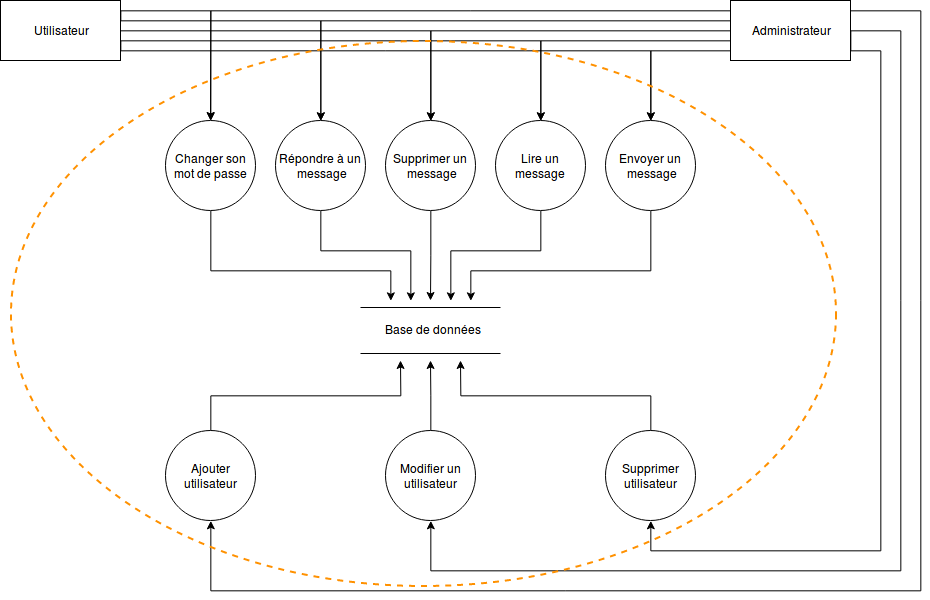
\includegraphics[width=480px]{diagram}
 	\caption{Diagramme de flux de données de l'application} 
 	\label{flux}	
\end{figure}


\subsection{Biens}
Les biens à protéger sont multiples dans une telle application. Ci-dessous, une liste non exhaustive de ces derniers

\begin{itemize}
\item Les messages 
\item Les comptes utilisateurs (leurs mots de passes)
\item Laccès à l'administration des comptes
\end{itemize}

%%%%%%%%%%%%%%%%%%%%%%%%%%%%%%%%%%%%%%%%%%%%%%%%%%%%%%%%%%%%%%%%%%%%%%%%%%%%%%%%%%%%%%%%%%%%%%
%%%%%%%%%%%%%%%%%%%%%%%%%%% SOURCES MENACES %%%%%%%%%%%%%%%%%%%%%%%%%%%%%%%%%%%%%%%%%%%%%%%%%%
%%%%%%%%%%%%%%%%%%%%%%%%%%%%%%%%%%%%%%%%%%%%%%%%%%%%%%%%%%%%%%%%%%%%%%%%%%%%%%%%%%%%%%%%%%%%%%
\newpage
\section{Sources de menaces}

\begin{tabular}{| l | l | l | c |}
  \hline			
  \textbf{Initiateur} & \textbf{Motivations} & \textbf{Cible(s)} & \textbf{Potentialité} \\
  \hline
  Utilisateur & Fun, Revanche, Curiosité & Tout éléments accessibles & Haute \\
  Administrateur & Revanche, Curiosité & Tout éléments accessibles & Moyenne \\  
  Concurrent & Secrets d'entreprise & Base de données & Moyenne \\
  Hackers & Gloire, Argent, Destruction & Tout éléments accessibles & Faible \\
  Cyber-criminel & Vol d'informations, Spam, DDoS & Base de données & Faible \\
  \hline  
\end{tabular}
\\

Parmi les différents initiateurs décrits ci-dessus, les utilisateurs représentent la plus grande menace et la menace la plus probable d'arriver. En effet, comme le programme est destiné à un usage interne à l'entreprise, a priori seuls les employés y auront accès.

N'y avoir accès que en interne ne signifie pas que ce n'est pas accessible de l'extérieur. Un attaquant externe (hacker, concurrent, cybercriminel) pourra tout à fait utiliser de l'ingénierie sociale pour inciter un utilisateur à lancer un programme malveillant afin de rendre l'accès à distance possible par le biais d'un reverse shell par exemple.  

%%%%%%%%%%%%%%%%%%%%%%%%%%%%%%%%%%%%%%%%%%%%%%%%%%%%%%%%%%%%%%%%%%%%%%%%%%%%%%%%%%%%%%%%%%%%%%
%%%%%%%%%%%%%%%%%%%%%%%%%%% SCENARIOS D'ATTAQUE %%%%%%%%%%%%%%%%%%%%%%%%%%%%%%%%%%%%%%%%%%%%%%
%%%%%%%%%%%%%%%%%%%%%%%%%%%%%%%%%%%%%%%%%%%%%%%%%%%%%%%%%%%%%%%%%%%%%%%%%%%%%%%%%%%%%%%%%%%%%%
\newpage
\section{Scénarios d'attaques}

Dans cette section, plusieurs scénarios d'attaque sont décrits. Grâce à ces scénarios, il est possible d'imaginer les différents points vulnérables de l'application et ainsi permet de mettre en place des contremesures appropriées.

\begin{tabular}{| c | l | p{6.5cm} | l |}
  \hline			
  \textbf{\# }& \textbf{Impact} &\textbf{ Source de menace } & \textbf{Bien ciblé} \\
  \hline  
  \ref{1} & Perte de confidentialité & Utilisateur, Concurrent, Hacker, Cyber-criminel & BDD \\
    \hline  
  \ref{2} & Perte de disponibilité & Tous & Tout élément actif \\
    \hline  
  \ref{3} & Perte d'intégrité & Hacker, Concurrent & BDD \\
  \hline  

\end{tabular}

\subsubsection{Scénario d'attaque} \label{1}
Dans ce scénario d'attaque, les différents acteurs listés en tant que source de menace tenteront d'accèder à des informations qui ne leurs sont pas destinées. Pour parvenir à ses fins, un attaquant pourra essayer de multiples vecteurs d'attaque tels que : 

\begin{itemize}
\item Manipulation de l'URL
\item Injection SQL dans les divers champs de saisie disponibles
\item Utilisation d'une faille de XSS stocké afin de récupérer des cookie de session
\end{itemize}

Sans aucunes 

Avec peu de recherches sur internet et quelques tentatives, un attaquant avec de faibles connaissances sera en mesure de récupérer des données confidentielles tels que des mails ou encore des mots de passes en utilisant une injection SQL.

Avec une attaque plus élaborée, cet employé pourrait récupérer des cookie de session en se servant d'une attaque par XSS. Un message avec du code php sera stocké sur le serveur et quand l'utilisateur cible se connectera à sa boîte de réception, le code malicieux sera exécuté.

\subsubsection{Scénario d'attaque} \label{2}
Ce scénario d'attaque est basé sur le scénario \ref{1}. En effet, des hackers, concurrents ou des cybercriminels pourraient être intéressés par les informations potentiellements confidentielles échangées entre les différents collaborateurs de l'entreprise.

Leurs motivations seraient en grande partie financières. En effet, un Hacker pourra faire par exemple du chantage à l'entreprise en menaçant de divulguer les informations récoltées. Un concurrent pourra se servir des informations obtenues afin de proposer des produits ou services similaires à ceux proposés par l'entreprise attaquée sans avoir à les développer.

Si le programme de messagerie développé n'est utilisé que sur un réseau interne, la première phase d'une attaque pour un attaquant externe serait de pénétrer le réseau interne de l'entreprise. Pour ce faire, de l'ingénierie sociale peut être tentée envers les collaborateurs par le biais de mails forgés et de pièces jointes malicieuses. Ce procédé sera à répéter pour chaques scénarios où les attaquants sont externes au réseau de l'entreprise.

\subsubsection{Scénario d'attaque} \label{3}


\subsubsection{Scénario d'attaque} \label{4}
Ce scénario concerne la destruction d'informations par des tiers tels que des hackers ou encore des concurrents. Plusieurs approches sont possibles : 

\begin{itemize}
\item Attaques XSS réfléchi ou stocké
\item Attaques CSRF
\item Injections SQL
\end{itemize}

Grâce à une attaque XSS, un attaquant pourra dérober les cookie de session d'un administrateur pour ensuite se connecter en son nom et supprimer des utilisateurs ou les basculer en inactif. 

Avec l'aide d'un peu d'ingénierie sociale, un attaquant pourrait forger un lien pour supprimer des utilisateurs ou des messages et ensuite inciter un administrateur a cliquer sur son lien. Afin de dissimuler le contenu du lien, des services tels que "google short url" peuvent être utilisés.

A l'aide d'une injection SQL, un attaquant pourrait complètement supprimer toutes les entrées dans la base de données ou encore faire des entrées arbitraires tels que ajouter des administrateurs, modifier des entrées, etc...

\subsubsection{Scénario d'attaque} \label{5}
\subsubsection{Scénario d'attaque} \label{6}

%%%%%%%%%%%%%%%%%%%%%%%%%%%%%%%%%%%%%%%%%%%%%%%%%%%%%%%%%%%%%%%%%%%%%%%%%%%%%%%%%%%%%%%%%%%%%%
%%%%%%%%%%%%%%%%%%%%%%%%%%% CONTREMESURES %%%%%%%%%%%%%%%%%%%%%%%%%%%%%%%%%%%%%%%%%%%%%%%%%%%%
%%%%%%%%%%%%%%%%%%%%%%%%%%%%%%%%%%%%%%%%%%%%%%%%%%%%%%%%%%%%%%%%%%%%%%%%%%%%%%%%%%%%%%%%%%%%%%
\section{Contremesures}

tableau récap et montrer new implémentation

\begin{tabular}{| c | c | p{6.5cm} | p{6.5cm} |}
  \hline			
  \textbf{\# }& \textbf{Scénario} &\textbf{ Vulnérabilité }& \textbf{Contremesure}\\
  \hline  
  \ref{c1} & \ref{1} & xxx & yyy\\
  \hline

\end{tabular}

\subsection{Contremesure}\label{c1}

\end{document}
